%!TEX program = xelatex
\documentclass[aspectratio=169]{beamer}
\usepackage[T1]{fontenc}
\usepackage{hyphenat}
\usepackage{geometry}
\usepackage{overpic}
\usepackage{tikz}
\usepackage{ulem}
\usepackage[export]{adjustbox}

\usetikzlibrary{arrows, positioning}

%----------------------------------------
% Theme
%----------------------------------------

\graphicspath{{images/}}

\usetheme{utbm}
%\usetheme[illustration=cover]{utbm} % use cover.png/jpg/... for the title page

%\useinnertheme[illustration=cover]{utbm}
%\useoutertheme{utbm}
%\usecolortheme{utbm}
%
\hypersetup{
    colorlinks=true,% make the links colored
    linkcolor=blue,
}

%----------------------------------------
% Informations
%----------------------------------------

\newcommand\TODO[1]{\textcolor{red}{TODO\@: #1}}

\title[Développement d’une plateforme de recueil de consentements RGPD]{Soutenance de stage}
\subtitle{Développement d’une plateforme de recueil de consentements RGPD}
\author{Nicolas Ballet}
\institute[UTBM]{Université de Technologie de Belfort Montbéliard}

\def\twodigits#1{\ifnum#1<10 0\fi\the#1}
\date[\the\year-\twodigits\month-\twodigits\day]{\today}

% PDF metadata informations
\keywords{Versusmind \hyp{} RGPD \hyp{} Consentement \hyp{} Signature numérique \hyp{} Cloud Microsoft Azure \hyp{} Méthodologie Scrum \hyp{} Azure DevOps \hyp{} Angular \hyp{} Spring Boot \hyp{} Azure Functions}
\subject{J'ai pu, durant mon stage de fin d'études à Versusmind (Strasbourg), participer au développement d'un plateforme de recueil de consentement hébergée dans le cloud Microsoft Azure. L'équipe dont j'ai fait partie, utilise la methode agile Scrum. J'ai aidé à terminer une refonte graphique, mais aussi, à faire face à des problèmatiques de montée en charge et d'optimisation. Le tout sur une base de tests d'intégrations à l'aide d'Azure DevOps.}

%----------------------------------------
% Document
%----------------------------------------
\begin{document}
\begin{frame}[plain,noframenumbering]
    \titlepage{}
\end{frame}
\begin{frame}[noframenumbering]
    \frametitle{Sommaire}
    \tableofcontents
\end{frame}

\section{Contexte}
\begin{frame}
    \frametitle{Introduction}
    \framesubtitle{Entreprise}
    \begin{columns}
        \hfill
        \begin{column}{.45\textwidth}
            \parbox[c][0.8\textheight][c]{\columnwidth}{
                \begin{center}
                    
\includegraphics[width=.8\textwidth]{versusmind.png}
                \end{center}
                \begin{center}
                    \color{gray} Cabinet d'architecture numérique\\
                    \scriptsize\color{gray}Nancy \hyp{} Metz \hyp{} Luxembourg \hyp{} Paris \hyp{} Strasbourg
                \end{center}
                
\includegraphics[width=.62\textwidth]{versusconsulting.png}
                
\includegraphics[width=.65\textwidth, right]{versusxperience.png}
                
\includegraphics[width=.55\textwidth]{versusinstitute.png}
            }
        \end{column}
        \begin{column}{.5\textwidth}
            \parbox[c][0.8\textheight][c]{\columnwidth}{
                \begin{center}
                    \frame{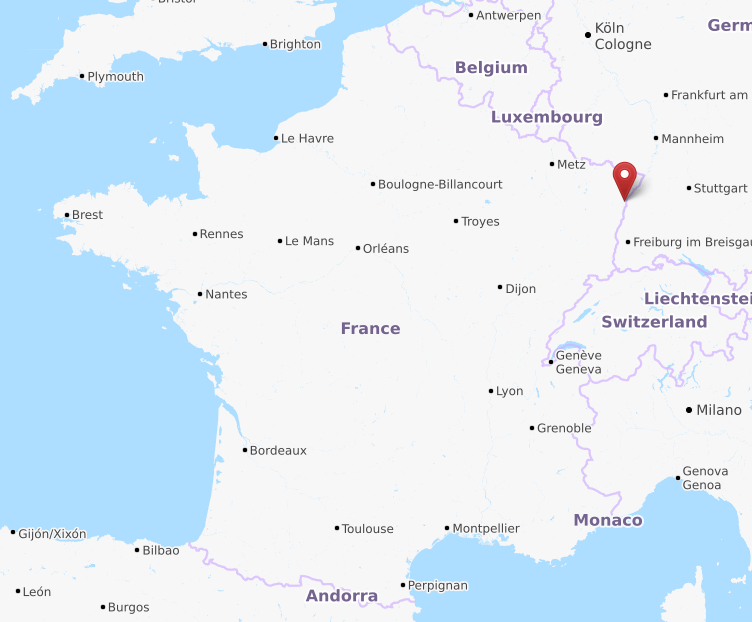
\includegraphics[width=1.0\textwidth]{strasbourg.png}}
                \end{center}
            }
        \end{column}
    \end{columns}
\end{frame}
\begin{frame}
    \frametitle{Introduction}
    \framesubtitle{RGPD}
    \begin{center}
        Règlement Général sur la Protection des Données
    \end{center}
    \begin{columns}
        \begin{column}{.45\textwidth}
            \parbox[c][0.6\textheight][c]{\columnwidth}{
                \begin{center}
                    \begin{enumerate}
                        \item<2-> Uniformiser la réglementation au niveau européen
                        \item<3-> Responsabiliser les entreprises
                        \item<4-> Renforcer les droits des personnes
                    \end{enumerate}
                \end{center}
            }
        \end{column}
        \begin{column}{.5\textwidth}
            \parbox[c][0.6\textheight][c]{\columnwidth}{
                \begin{center}
                    \only<1->{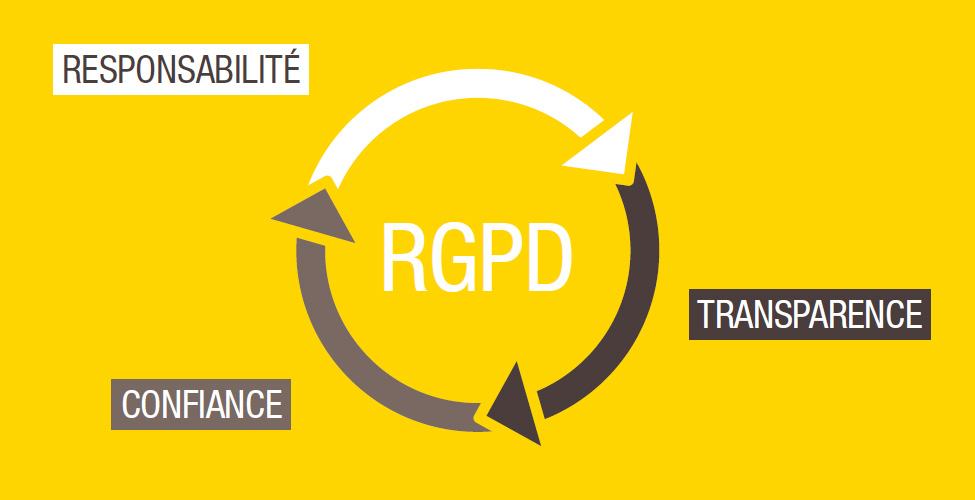
\includegraphics[width=1.0\textwidth]{RGPD.jpg}}
                \end{center}
            }
        \end{column}
    \end{columns}
\end{frame}
\begin{frame}
    \frametitle{Introduction}
    \framesubtitle{Central Consent Manager (CCM)}
    \hfill
    \begin{center}
        \onslide<2->{
\includegraphics[width=.4\textwidth]{ccm_.png}}
    \end{center}
    \begin{columns}
        \begin{column}{.45\textwidth}
            \parbox[c][0.5\textheight][c]{\columnwidth}{
                \begin{center}
                    
\includegraphics[width=.2\textwidth]{processing.png}\\
                    Tenir un registre des traitements de données personnelles
                \end{center}
            }
        \end{column}
        \begin{column}{.45\textwidth}
            \parbox[c][0.5\textheight][c]{\columnwidth}{
                \begin{center}
                    
\includegraphics[width=.2\textwidth]{consent.png}\\
                    Stocker les consentements
                \end{center}
            }
        \end{column}
    \end{columns}
\end{frame}
\begin{frame}
    \frametitle{Introduction}
    \framesubtitle{Central Consent Manager (CCM)}
    \begin{columns}
        \begin{column}{.45\textwidth}
            \parbox[c][0.8\textheight][c]{\columnwidth}{
                \begin{center}
                    \begin{enumerate}
                        \item<2-> Requête sur les informations d'un traitement
                        \item<3-> Envoi des informations du traitement
                        \item<4-> Demande de consentement
                        \item<5-> Confirmation
                        \item<6-> Enregistrement du consentement
                    \end{enumerate}
                \end{center}
            }
        \end{column}
        \begin{column}{.5\textwidth}
            \parbox[c][0.8\textheight][c]{\columnwidth}{
                \begin{center}
                    \only<1>{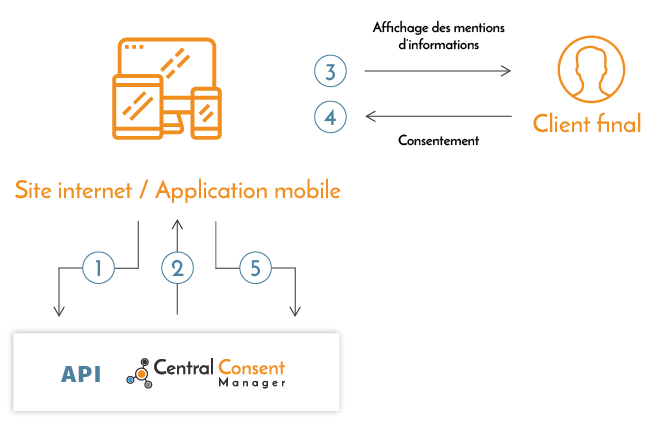
\includegraphics[width=1.0\textwidth]{ccm.png}\\}
                    \only<2>{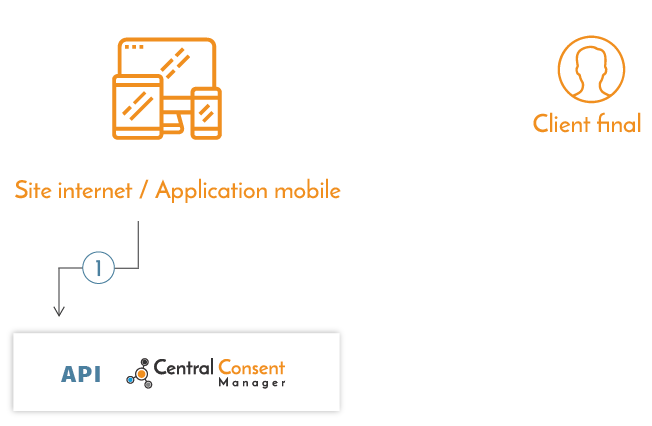
\includegraphics[width=1.0\textwidth]{ccm1.png}\\}
                    \only<3>{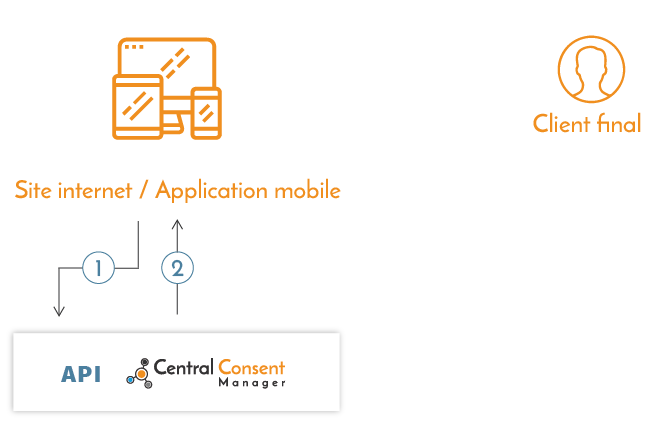
\includegraphics[width=1.0\textwidth]{ccm2.png}\\}
                    \only<4>{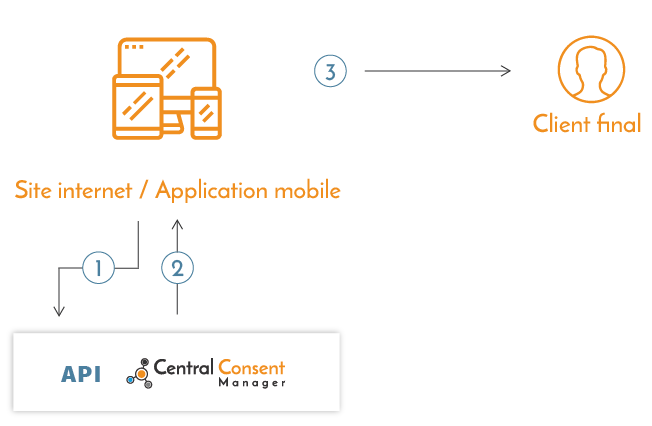
\includegraphics[width=1.0\textwidth]{ccm3.png}\\}
                    \only<5>{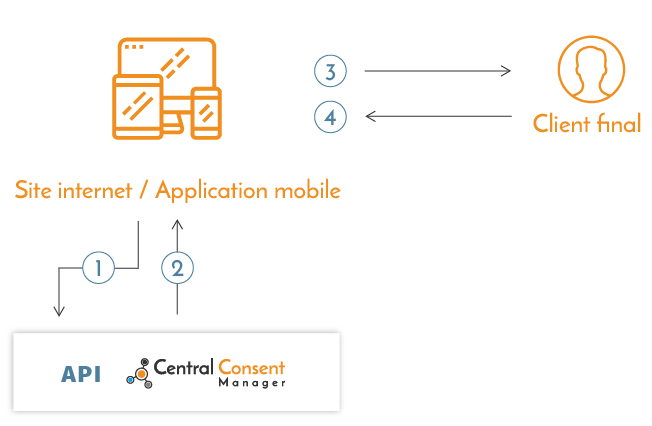
\includegraphics[width=1.0\textwidth]{ccm4.png}\\}
                    \only<6>{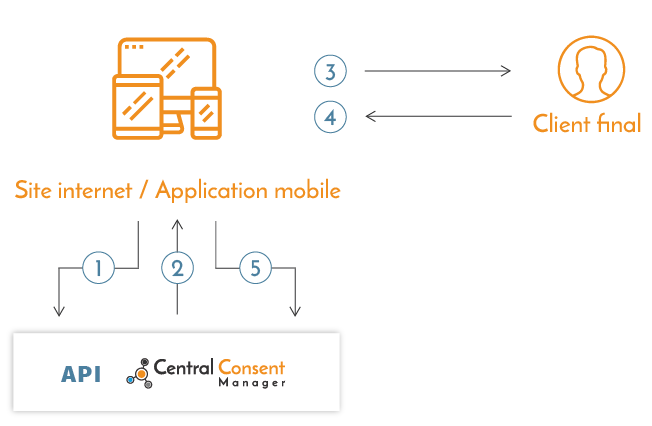
\includegraphics[width=1.0\textwidth]{ccm5.png}\\}
                \end{center}
            }
        \end{column}
    \end{columns}
\end{frame}

\section{Déroulé du stage}
\begin{frame}
    \frametitle{Transition}
    \framesubtitle{}
    \tableofcontents[currentsubsection,sectionstyle=show/shaded,subsectionstyle=show/shaded/hide]
\end{frame}
\begin{frame}
    \frametitle{Déroulé du stage}
    \framesubtitle{Refonte graphique}
    \begin{columns}
        \begin{column}{.4\textwidth}
            \parbox[c][0.8\textheight][c]{\columnwidth}{
                \begin{center}
                    \begin{itemize}
                        \item<2-> Redéfinition de l'expérience utilisateur
                        \item<3-> Unification de la charte graphique
                    \end{itemize}
                \end{center}
            }
        \end{column}
        \begin{column}{.55\textwidth}
            \parbox[c][0.8\textheight][c]{\columnwidth}{
                \begin{center}
                    \only<1-2>{\frame{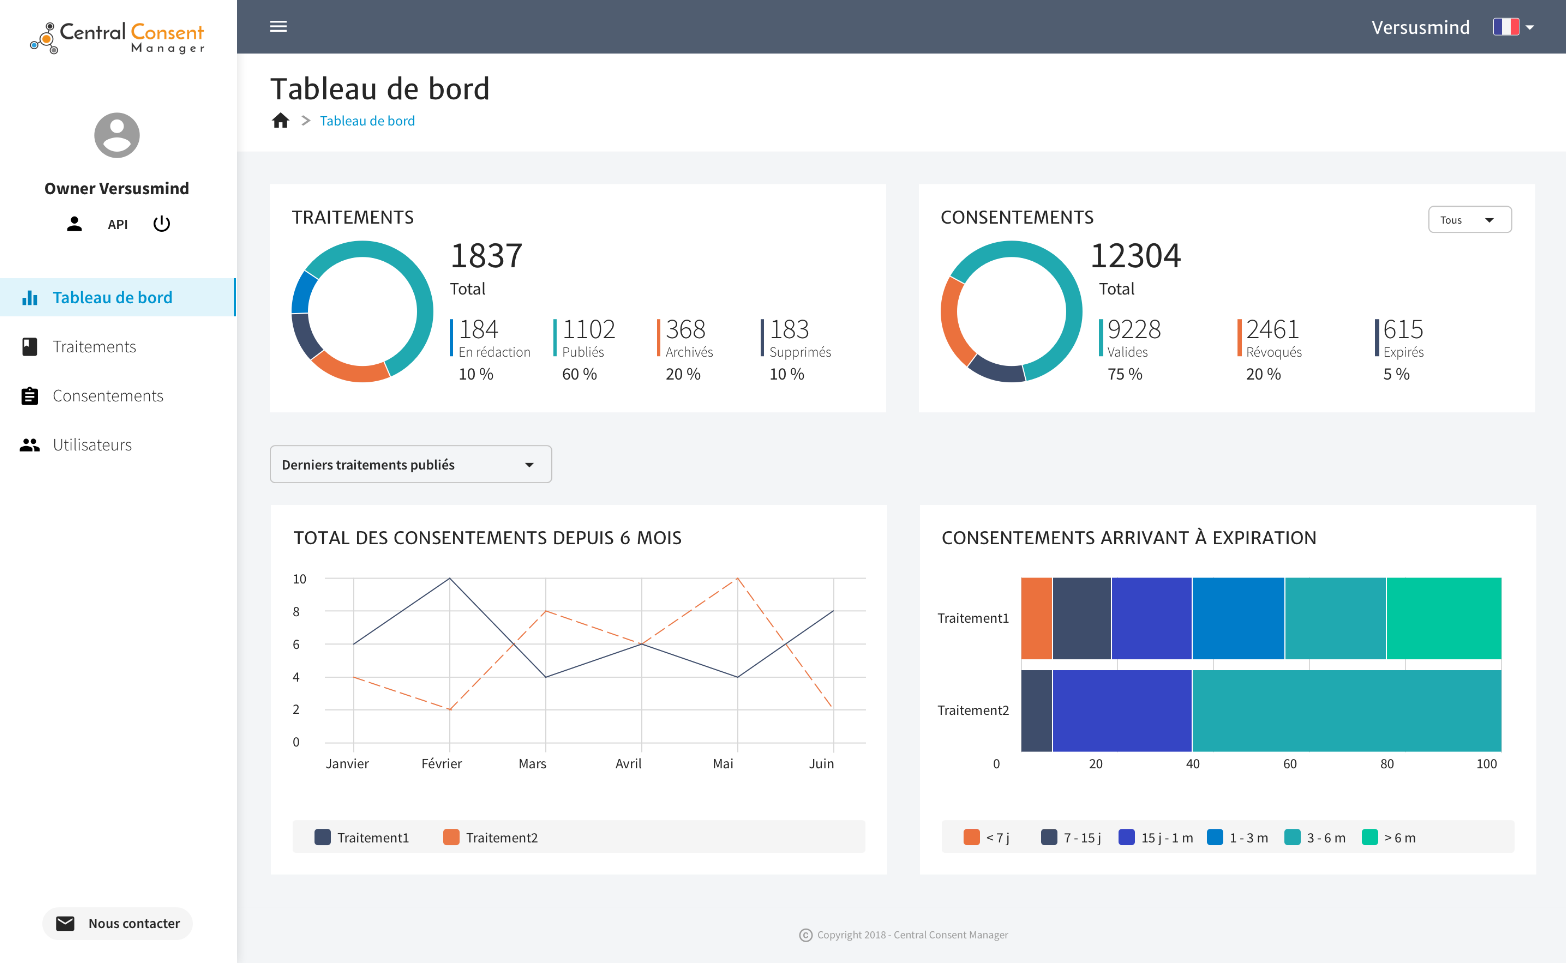
\includegraphics[width=1.0\textwidth]{dashboard.png}}}
                    \only<3>{\frame{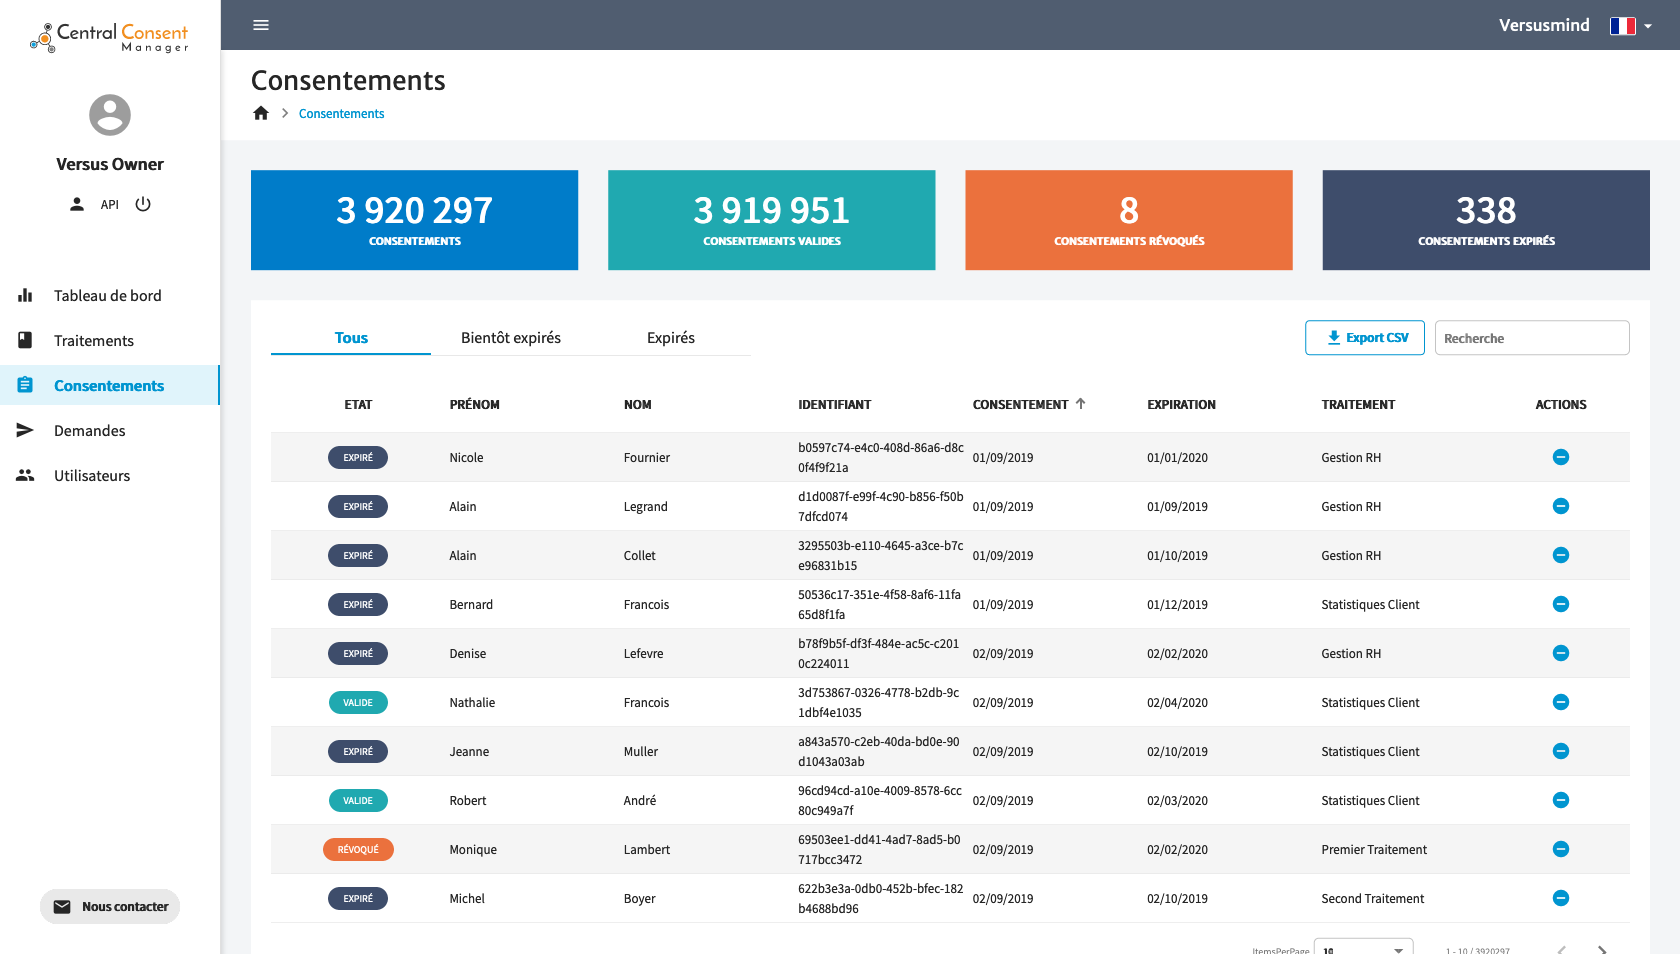
\includegraphics[width=1.0\textwidth]{consent_list.png}}}
                \end{center}
            }
        \end{column}
    \end{columns}
\end{frame}
\begin{frame}
    \frametitle{Déroulé du stage}
    \framesubtitle{Optimisation}
    \begin{center}
        \begin{tikzpicture}
            % nodes
            \node (api) at (1, 1.8) {
\includegraphics[width=.1\textwidth]{website.png}};
            \node [above=0 of api] {API};
            \node (front) at (1, -1.8) {\begin{overpic}[width=.1\textwidth]{website.png}
                    \put(60, -30){
\includegraphics[scale=.08]{ccm_logo.png}}
                \end{overpic}};
            \node [above=0 of front] {Front-end};
            \node (back) at (6, 0) {
\includegraphics[width=.1\textwidth]{server.png}};
            \node [above=0 of back] {Back-end};
            \node (function) at (12, 1.8) {\only<3->{
\includegraphics[width=.1\textwidth]{cloud.png}}};
            \node [above=0 of function] {\only<3->{Azure Function}};
            \node (ejbca) at (12, -2) {
\includegraphics[width=.2\textwidth]{ejbca.png}};
            \node (stats1) at (6, -1.7) {
                \only<2-4>{1M de consentements = 3 jours}
                \only<5->{\sout{1M de consentements = 3 jours}}
            };
            \node (stats2) at (6, -2.3) {\only<5->{1M de consentements = 40 minutes}};

            % arrows
            \only<1->{\draw[ultra thick, ->,>=stealth] (api) -- (back)};
            \only<1->{\draw[ultra thick, ->,>=stealth] (front) -- (back)};
            \only<1-2>{\draw[ultra thick, ->,>=stealth] (back) -- (ejbca)};
            \only<3>{\draw[ultra thick, double, <->,>=stealth] (back) -- node[above, sloped] {Service Bus} (function)};
            \only<4->{\draw[ultra thick, double, <->,>=stealth] (back) -- node[near start, below, sloped] {
\includegraphics[width=.05\textwidth]{paquet.png} lots} node[above, sloped] {Service Bus} (function)};
            \only<3->{\draw[ultra thick, ->,>=stealth] (function) -- (ejbca)};

        \end{tikzpicture}
    \end{center}
\end{frame}

\section{Ressenti personnel}
\begin{frame}
    \frametitle{Transition}
    \framesubtitle{}
    \tableofcontents[currentsubsection,sectionstyle=show/shaded,subsectionstyle=show/shaded/hide]
\end{frame}
\begin{frame}
    \frametitle{Ressenti personnel}
    \framesubtitle{}
    \begin{columns}
        \begin{column}{.5\textwidth}
            \parbox[c][0.8\textheight][c]{\columnwidth}{
                \begin{center}
                    \begin{itemize}
                        \item<1->{Environnement de travail agréable et équipe conviviale}
                        \item<2->{Pratique d'une méthode Agile (Scrum)}
                        \item<3->{Familiarisation avec les outils DevOps et le cloud Azure}
                        \item<4->{Proposition de CDI en tant que consultant}
                    \end{itemize}
                \end{center}
            }
        \end{column}
        \begin{column}{.44\textwidth}
            \parbox[c][0.8\textheight][c]{\columnwidth}{
                \begin{center}
                    \only<1>{\frame{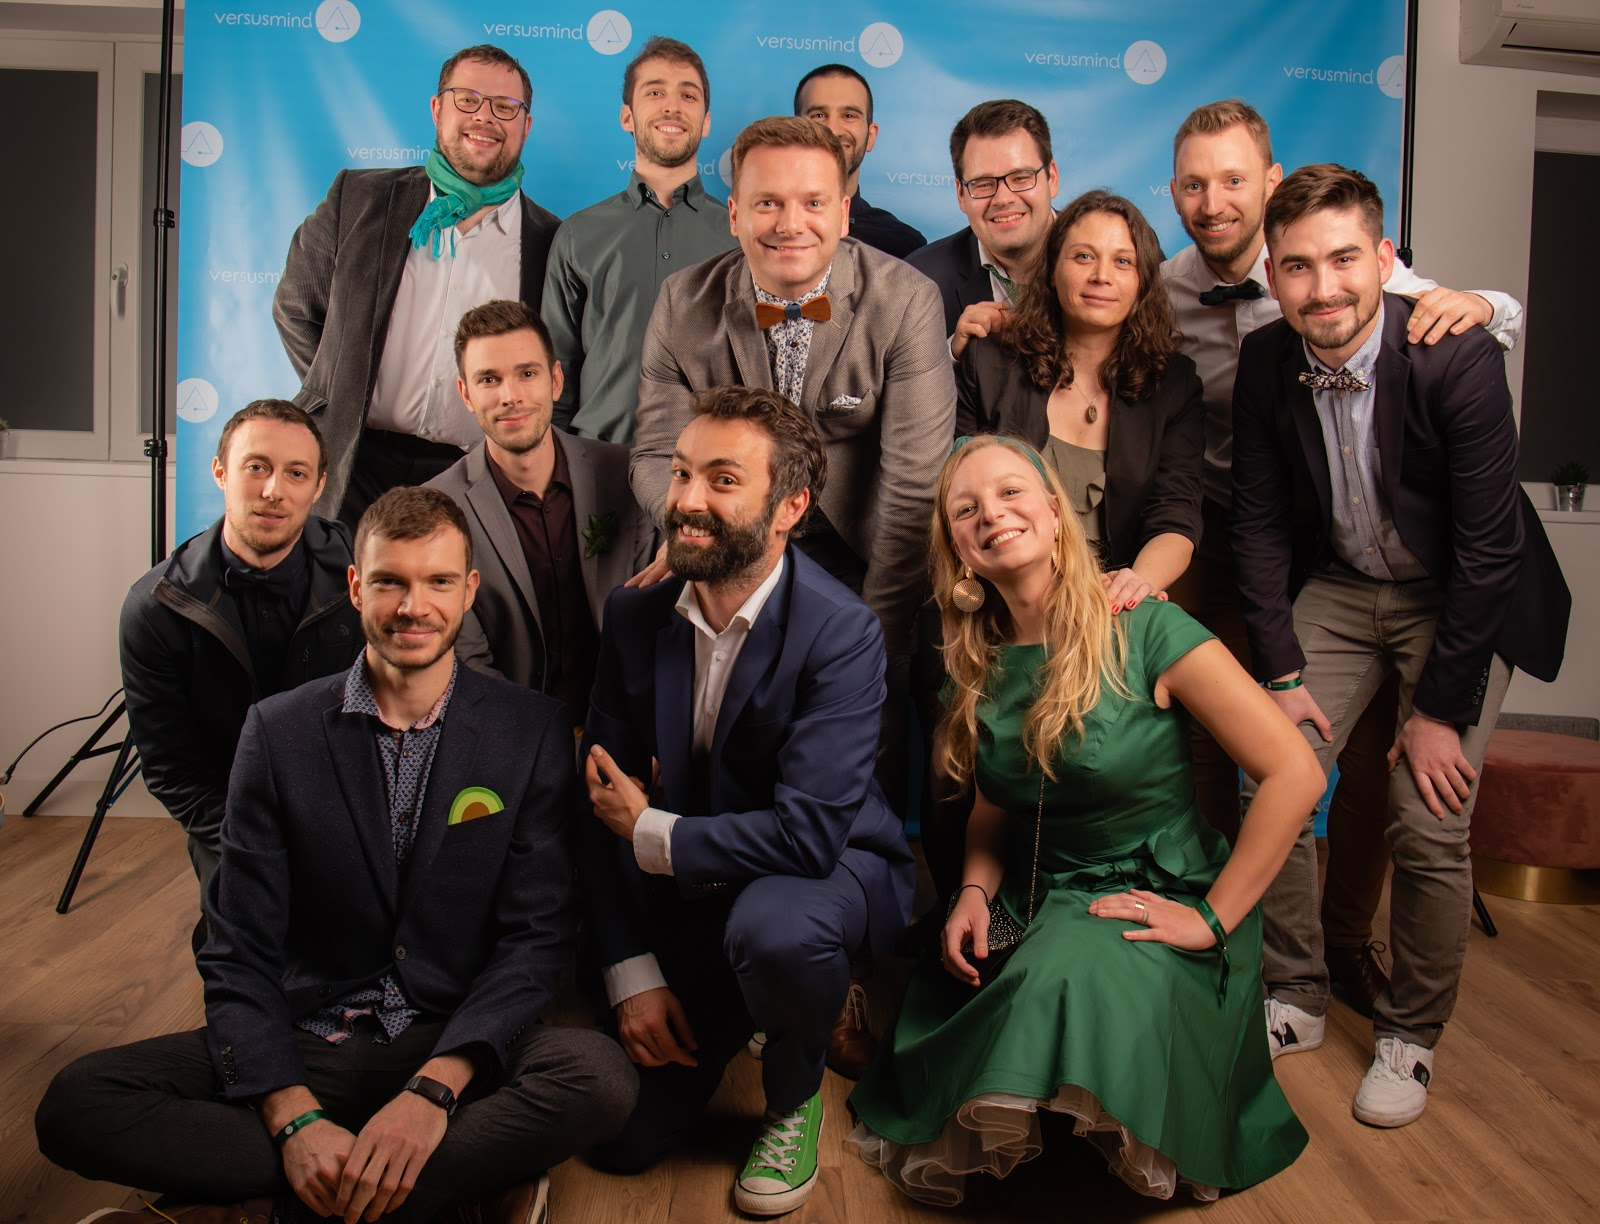
\includegraphics[width=\textwidth]{equipe.jpg}}\\}
                    \only<2>{\frame{
\includegraphics[width=0.5\textwidth]{livre_scrum.jpg}}}
                    \only<3>{
\includegraphics[width=\textwidth]{microsoft-azure.png}\\}
                    \only<4>{
\includegraphics[width=\textwidth]{cdi.png}\\}
                \end{center}
            }
        \end{column}
    \end{columns}
\end{frame}
\begin{frame}[plain,noframenumbering]
    \utbmclosingframe{Avez vous des questions ?}
\end{frame}
\end{document}
